%! Tex program = pdflatex
 
\documentclass[UTF8]{ctexart}
\CTEXsetup[format={\Large\bfseries}]{section}
\usepackage{amsmath}
\usepackage{ctex}
\usepackage{array}
\usepackage{ulem}
\usepackage{graphicx}
\usepackage{geometry}
\usepackage{multirow}
\usepackage{subfig}
\usepackage{float}
\usepackage{multicol}
\usepackage{multirow}
\usepackage{indentfirst}
\usepackage{makecell}
\geometry{papersize={21cm,29.7cm}}
\geometry{left=2.54cm,right=2.54cm,top=3.18cm,bottom=3.18cm}
\usepackage{fancyhdr}
\pagestyle{fancy}
\lhead{\today}
\chead{}
\rhead{2020011075}
\lfoot{清华大学}
\cfoot{\thepage}
\rfoot{物理实验B(2)}
\renewcommand{\headrulewidth}{0.4pt}
\renewcommand{\headwidth}{\textwidth}
\renewcommand{\footrulewidth}{0pt}
\usepackage{bm}
\begin{document}
\begin{titlepage}
    \begin{center}
		\quad \\
		\quad \\
        \quad \\
        \quad \\
        \quad \\
        \quad \\
		\kaishu \fontsize{30}{15} 偏振光学实验
	\end{center}
	\vskip 10cm

    \begin{center}
        \begin{large}
        \begin{tabular}{cc}
        院\qquad 系:& ~~~~~~~~自动化系~~~~~~~~      \\
        \cline{2-2}\\
        班\qquad 级:& 自02班   \\
        \cline{2-2}\\
        学生姓名:& 彭程    \\
        \cline{2-2}\\
        学\qquad 号:&2020011075   \\
        \cline{2-2}\\
        组\qquad 号:& 双四下L    \\
        \cline{2-2}\\
        座~~位~~号:& \# 5    \\
        \cline{2-2}
        \end{tabular}
        \end{large}
        \end{center}

\end{titlepage}
\newpage
\tableofcontents
\newpage
\section{实验名称}
偏振光学实验
\section{数据处理}
\subsection{观察激光束的偏振特性}

\noindent 记录光强极小时起偏器的度盘读数为:$34^\circ$,$215^\circ$。

\subsection{观察布氏角、定起偏器P的投射轴方向}

\noindent 1.观察布氏角

\noindent(1)光束正入射反射镜平面时平台方位角:$\alpha_{i=0}=108.4^\circ$

\noindent (2)观测布儒斯特角、起偏器P投射轴方向:

\begin{figure}[H]
  \centering
  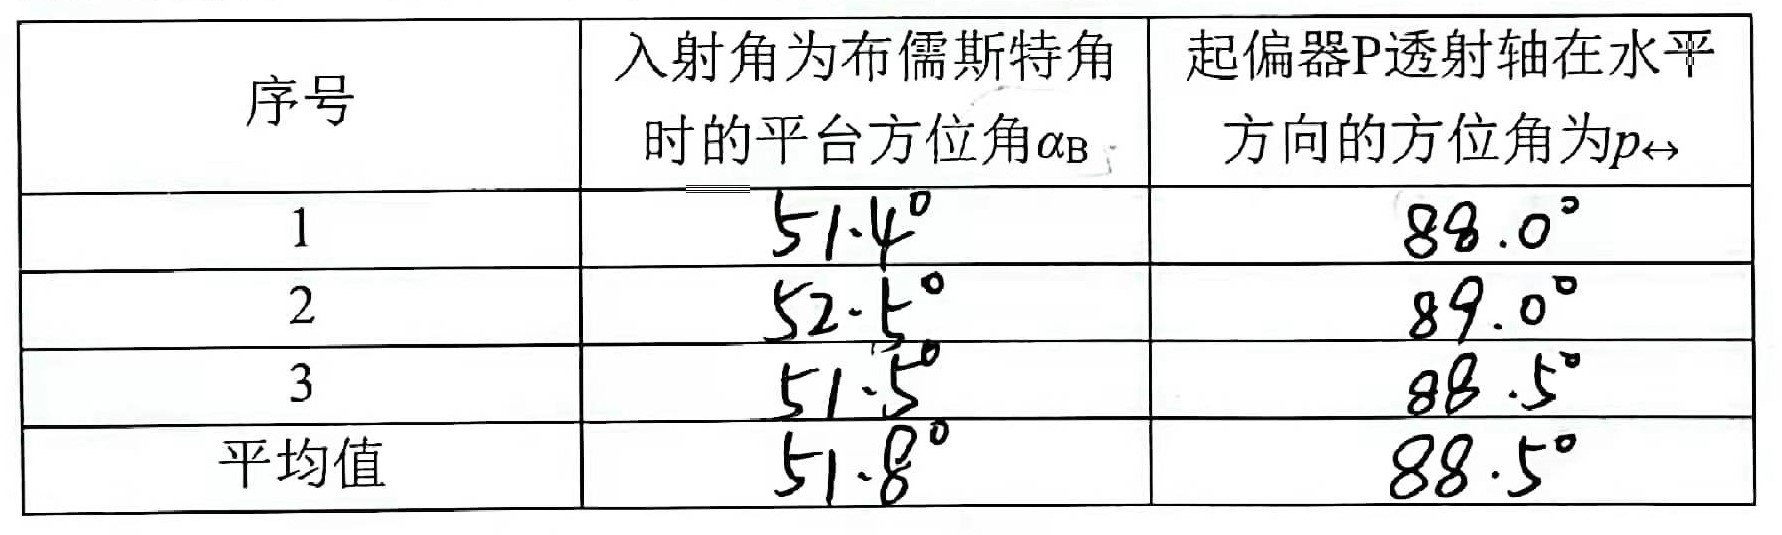
\includegraphics[scale=0.2]{5.jpg}
\end{figure}

布儒斯特角测量值$\theta_B=\overline{\alpha_B}-\alpha_{i=0}=56.6^\circ$

折射率$n=tan\theta_B=1.52$

\noindent 2.定检偏轴的投射轴方向:

检偏器A的投射轴位于垂直方向:$\alpha_{\updownarrow}={5.0}^\circ$



\subsection{测消光比}
交替测量透射光强极值:
\begin{figure}[H]
  \centering
  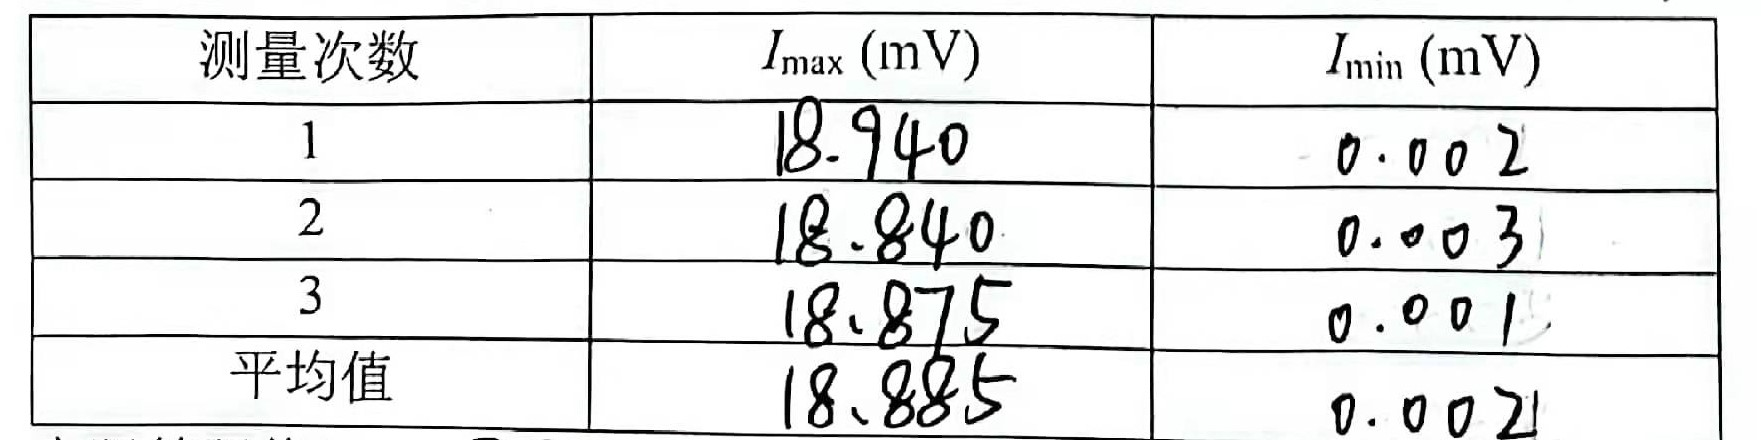
\includegraphics[scale=0.2]{6.jpg}
\end{figure}
电阻箱阻值:$R=200\Omega$

挡住光源时:$I_0=-0.007mV$

计算得到消光比为:$e=\frac{\overline{I_{min}}-I_0}{2\overline{I_{max}}}=0.0002$

\subsection{测量透射光强 $I_m$和两偏振器夹角$\theta$间的关系}

电阻箱示值:$R=200\Omega$,$p=\overline{p_{\leftrightarrow}}=88.5^\circ$,$\alpha_{\updownarrow}={5.0}^\circ$,挡住光源时:$I_0=-0.006mV$

保持起偏器P水平,转动检偏器A,测量经过A的出射光强:

\begin{figure}[H]
  \centering
  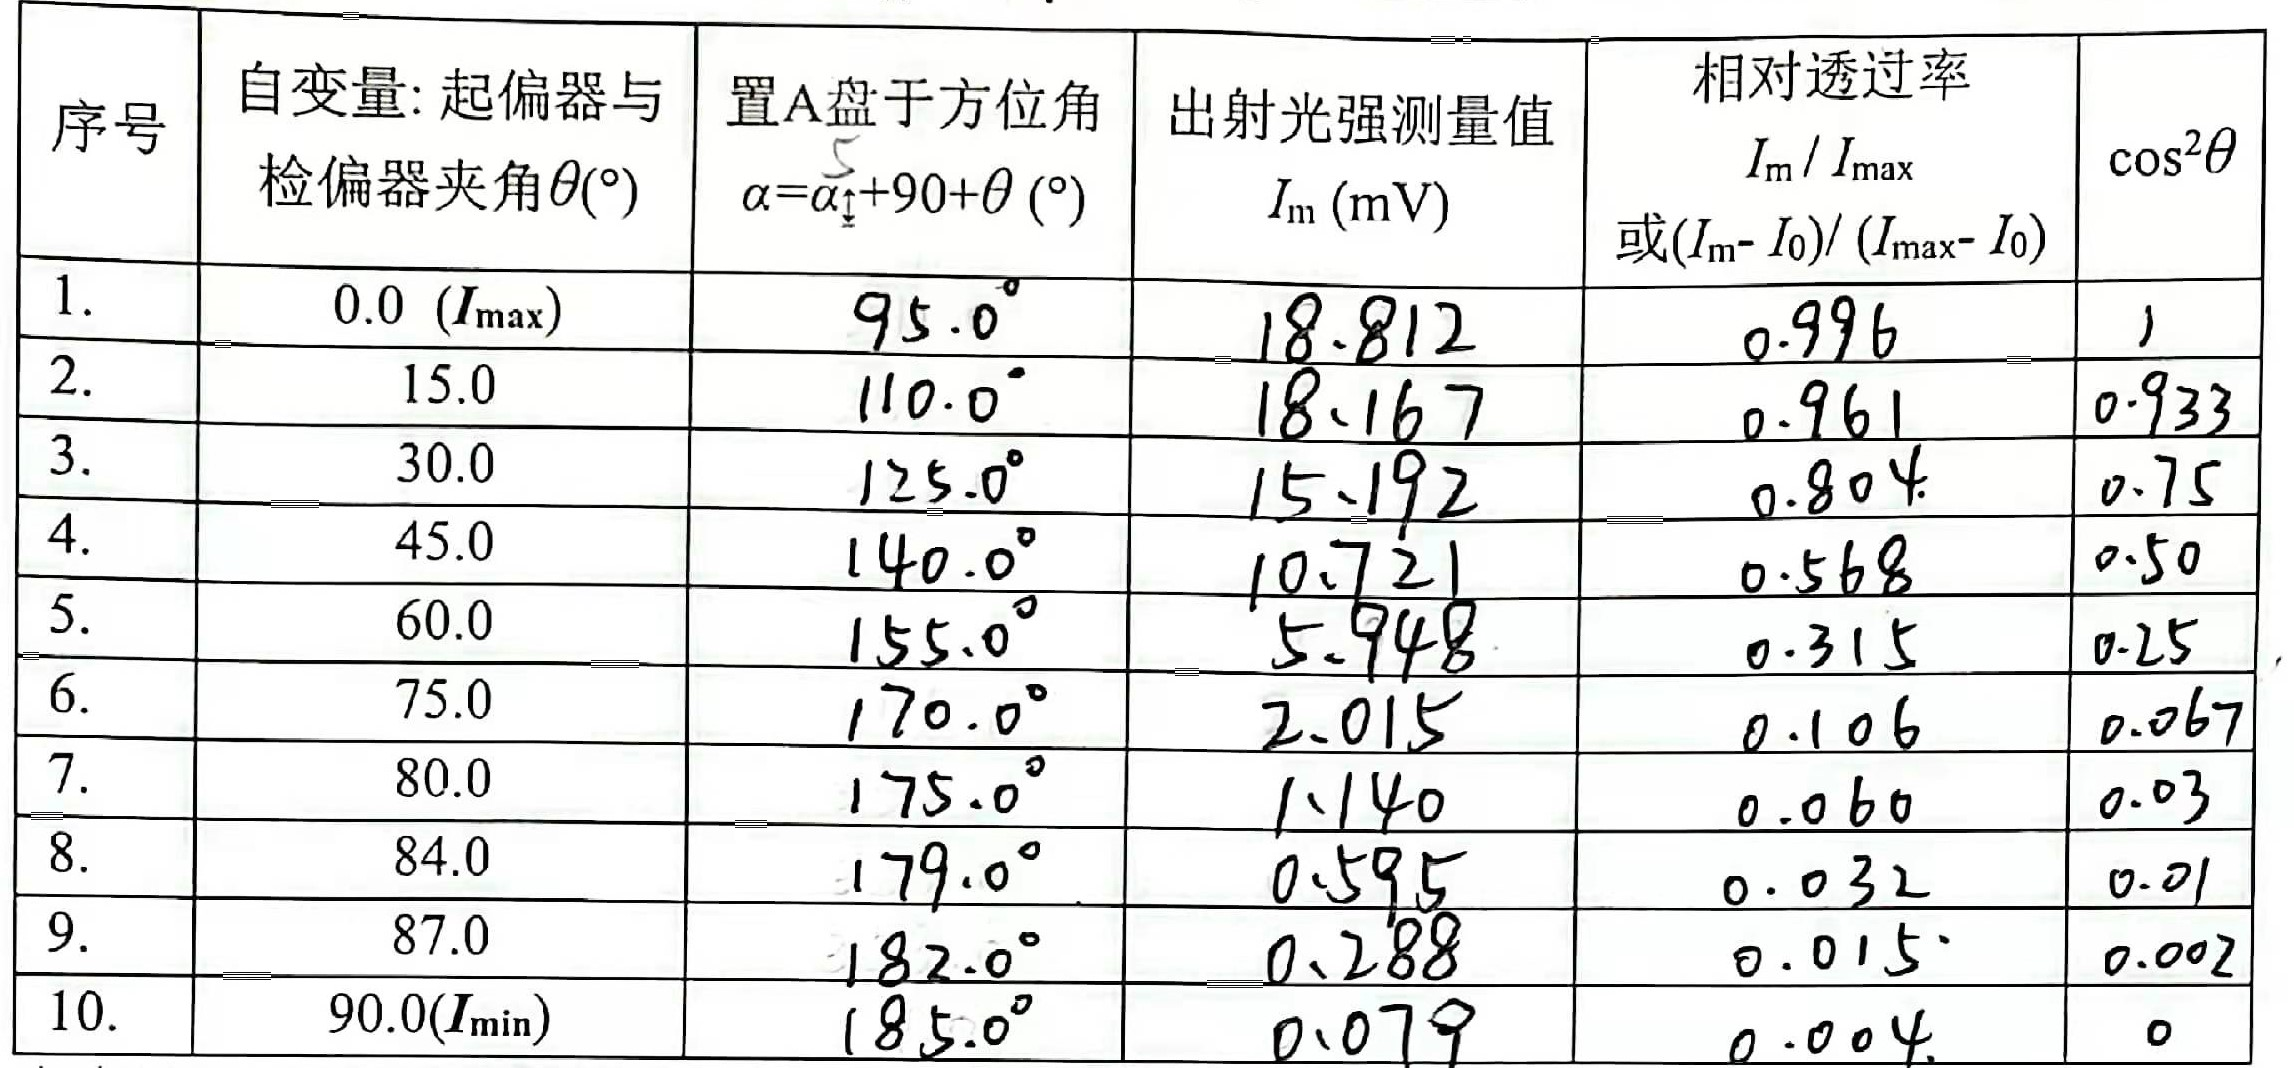
\includegraphics[scale=0.2]{7.jpg}
\end{figure}

绘制相对透射率随$\theta$变化的关系曲线:

\begin{figure}[H]
  \centering
  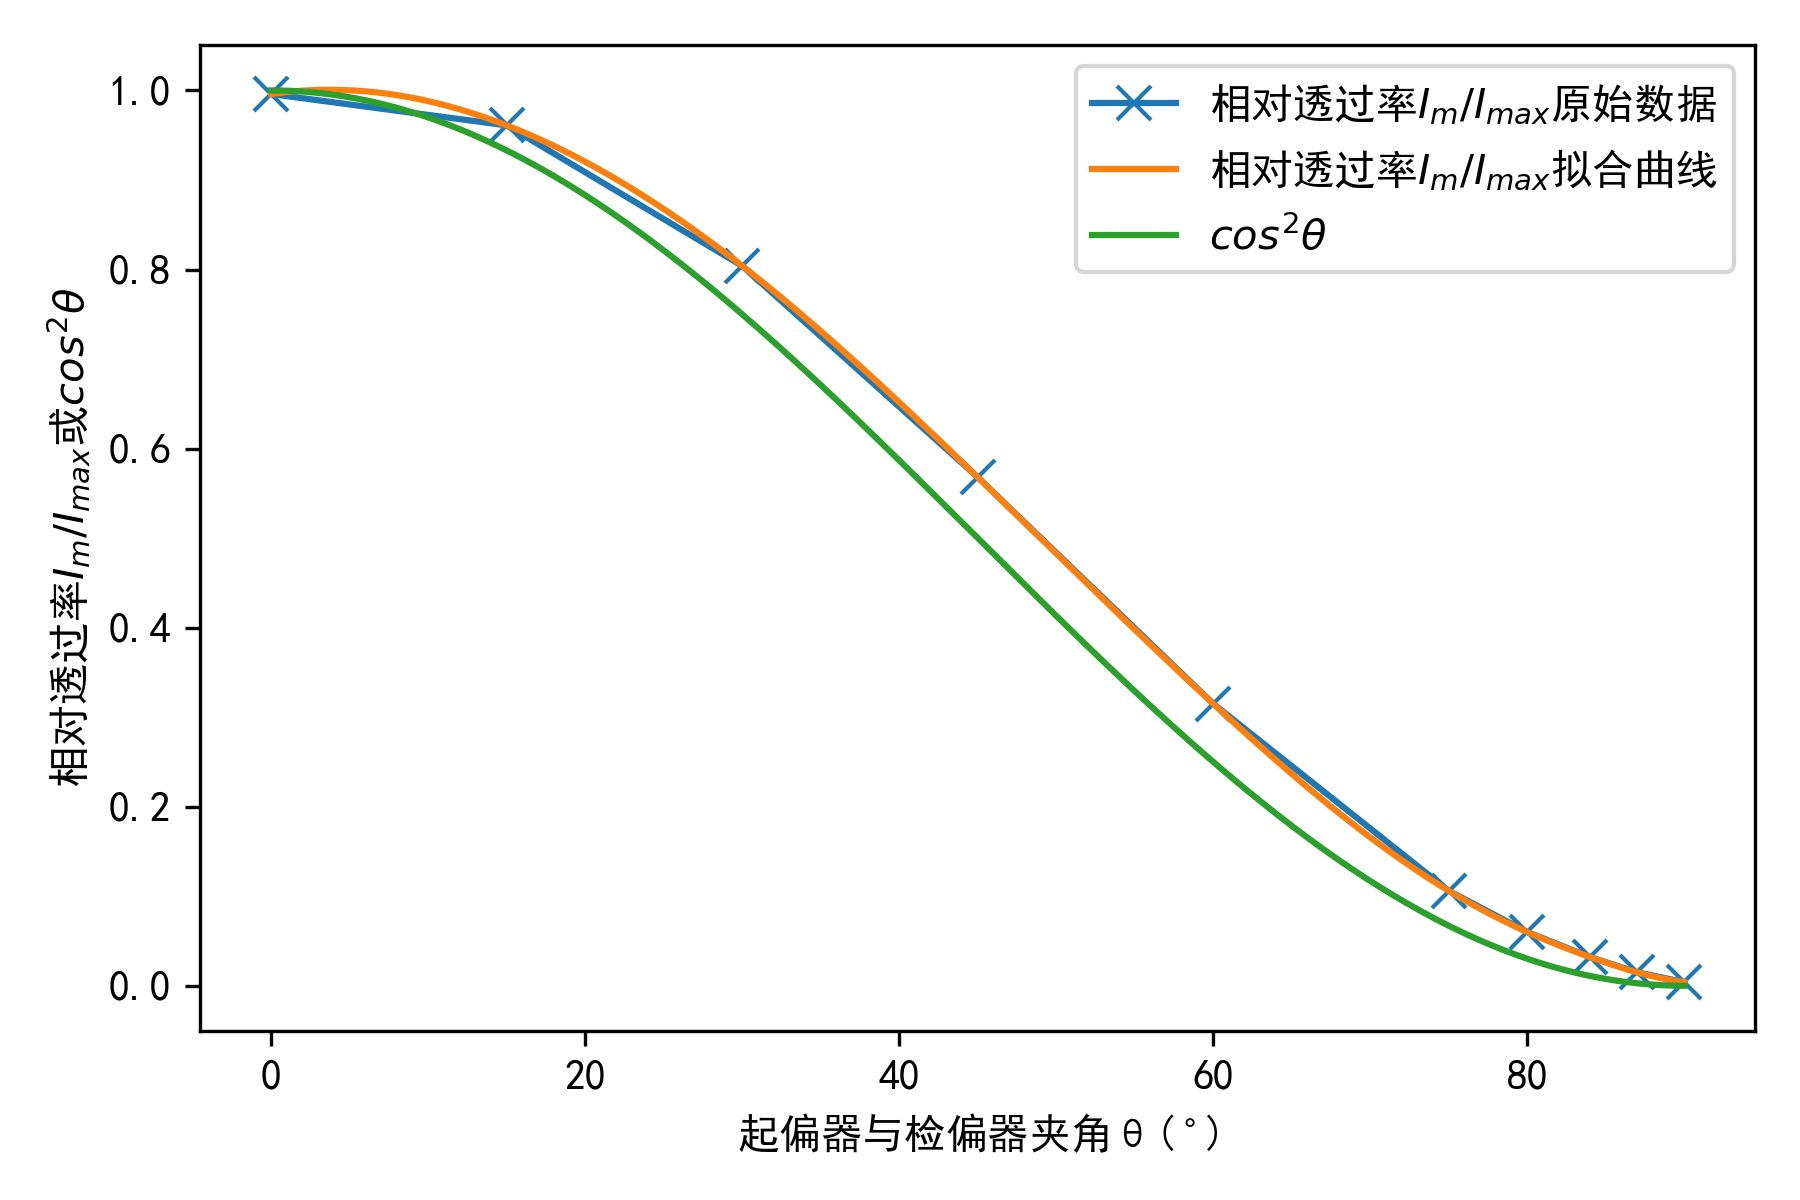
\includegraphics[scale=0.8]{8.jpg}
\end{figure}

观察发现相对透射率变化趋势和$cos^2\theta$变化趋势基本一致,比较符合马吕斯定律。

\subsection{定待测波片$ C_x$ 的轴向}

起偏器置于水平方向:$p=\overline{p_{\leftrightarrow}}=88.5^\circ$

检偏器A的投射轴位于垂直方向:$\alpha_{\updownarrow}={5.0}^\circ$

将待测波片置于平台,转动使三者消光,得$C_x$的一个轴在垂直方向时的度盘示值$c_x=334^\circ$



\subsection{定波片 $C_0$ 的快轴方向}
移去$C_x$,装上$C_0$,转动使三者消光,得$C_0$的快轴在垂直方向时的方位角$c_0=198^\circ$



\subsection{ 线偏振光经过 1/4 波片}


起偏器P投射轴位于水平方向$\overline{p_{\leftrightarrow}}=88.5^\circ$,波片$C_0$度盘示值$c_0=198^\circ$

改变起偏器投射轴与波片慢轴之间夹角,转动检偏器,测出长轴方位角和光强极大值、极小值。

\begin{figure}[H]
  \centering
  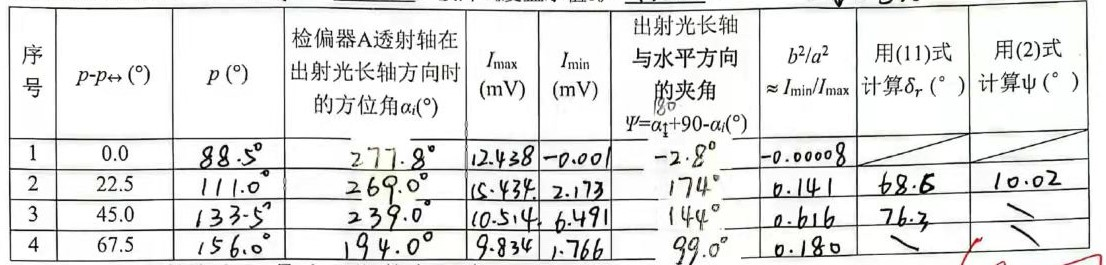
\includegraphics[scale=0.5]{9.jpg}
\end{figure}

理论上$\beta=0^\circ$近似于线偏振光,$\beta=45^\circ$近似于圆偏振光,此处实验有一定误差,可能是偏振片各区域透射度不同导致。

\subsection{偏振光通过 1/2 波片或全波片}

$C_x$的某轴在垂直方向,盘示值$c_x=331.0^\circ$;

$C_0$的快轴在垂直方向,度盘示值$c_0=198.0^\circ$;

起偏器和检偏器消光时旋向相反,说明是1/2波片。

\begin{figure}[H]
  \centering
  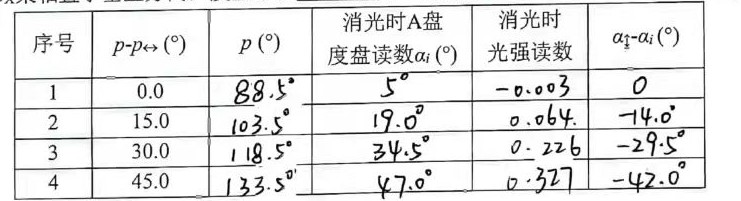
\includegraphics[scale=0.5]{10.jpg}
\end{figure}




$C_x$的某轴在垂直方向,盘示值$c_x=331.0^\circ$;

$C_0$的快轴转动$90^\circ$至水平方向,度盘示值$c_0=288.0^\circ$;

起偏器和检偏器消光时旋向相同,说明是全波片。
\begin{figure}[H]
  \centering
  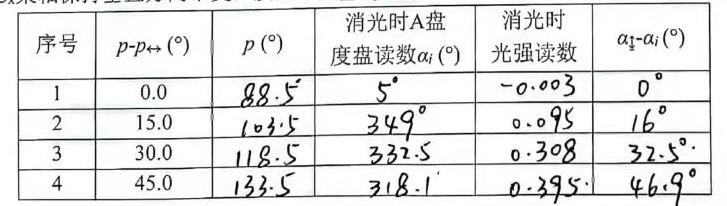
\includegraphics[scale=0.5]{11.jpg}
\end{figure}


\section{实验总结以及建议}

通过本实验,我认识到了半定量实验这种实验方式,在测量过程中,可能会由于各种原因对实验结果带来较大的误差,但通过实验数据,仍然能够观察出相关性质、验证相关定理、理解变化趋势,对于我认识相关理论和性质有比较好的帮助作用。

此外在本次实验中我还复习了上学期所学的有关偏振的相关理论内容,包括布儒斯特角、消光比、马吕斯
定律、 1/4 波片、 1/2 波片、全波片、各种偏振光的性质等。这一实验也让我对偏振光学的理解进
一步加深。

在实验之余,我对物理实验的课程设计有一点小小的建议,作为自动化的同学,在大一下学期时已经完成了对于电路原理、电路原理实验两门基础课的先修,所以在大二上的时候,有关示波器的原理和使用、直流电桥测电阻等实验均已有相关实验经历,故建议对于电学专业的同学的电学实验进行较为个性化的设计,希望我的建议对物理实验的课程改革有所帮助。

最后,感谢老师对我们的悉心指导!

\section{原始数据}

\begin{figure}[H]
  \centering
  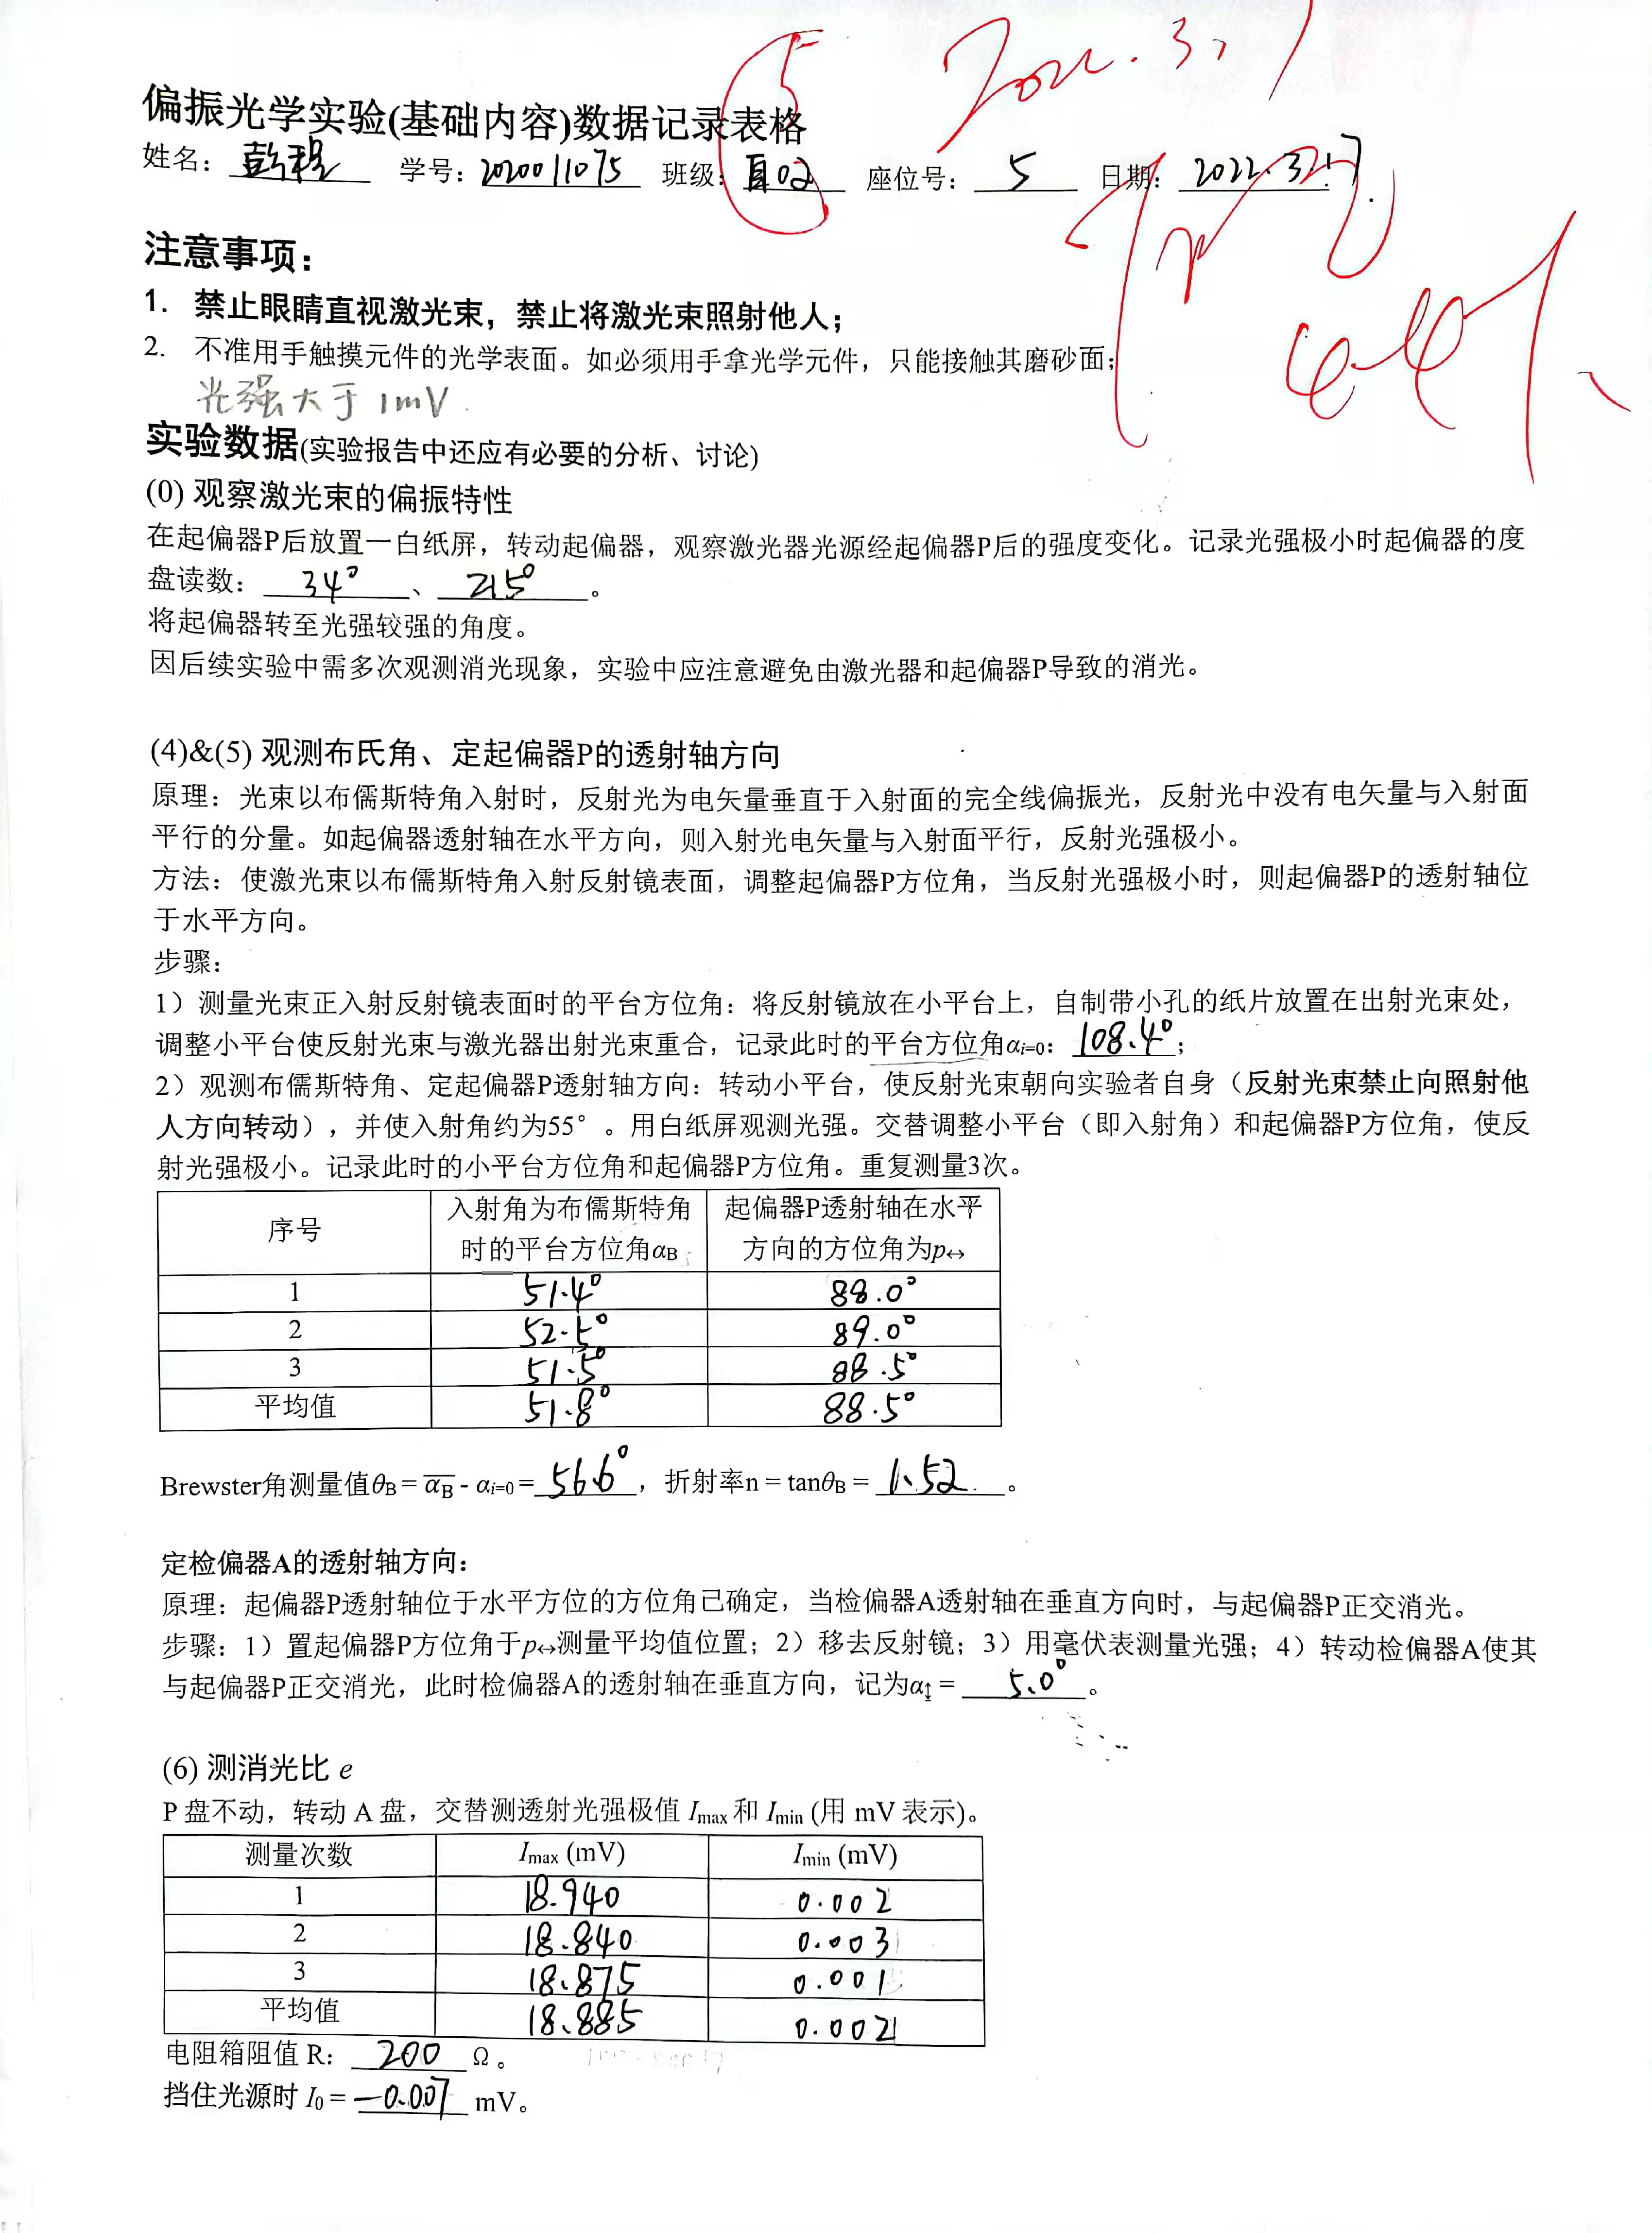
\includegraphics[scale=0.13]{1.jpg}
\end{figure}

\begin{figure}[H]
  \centering
  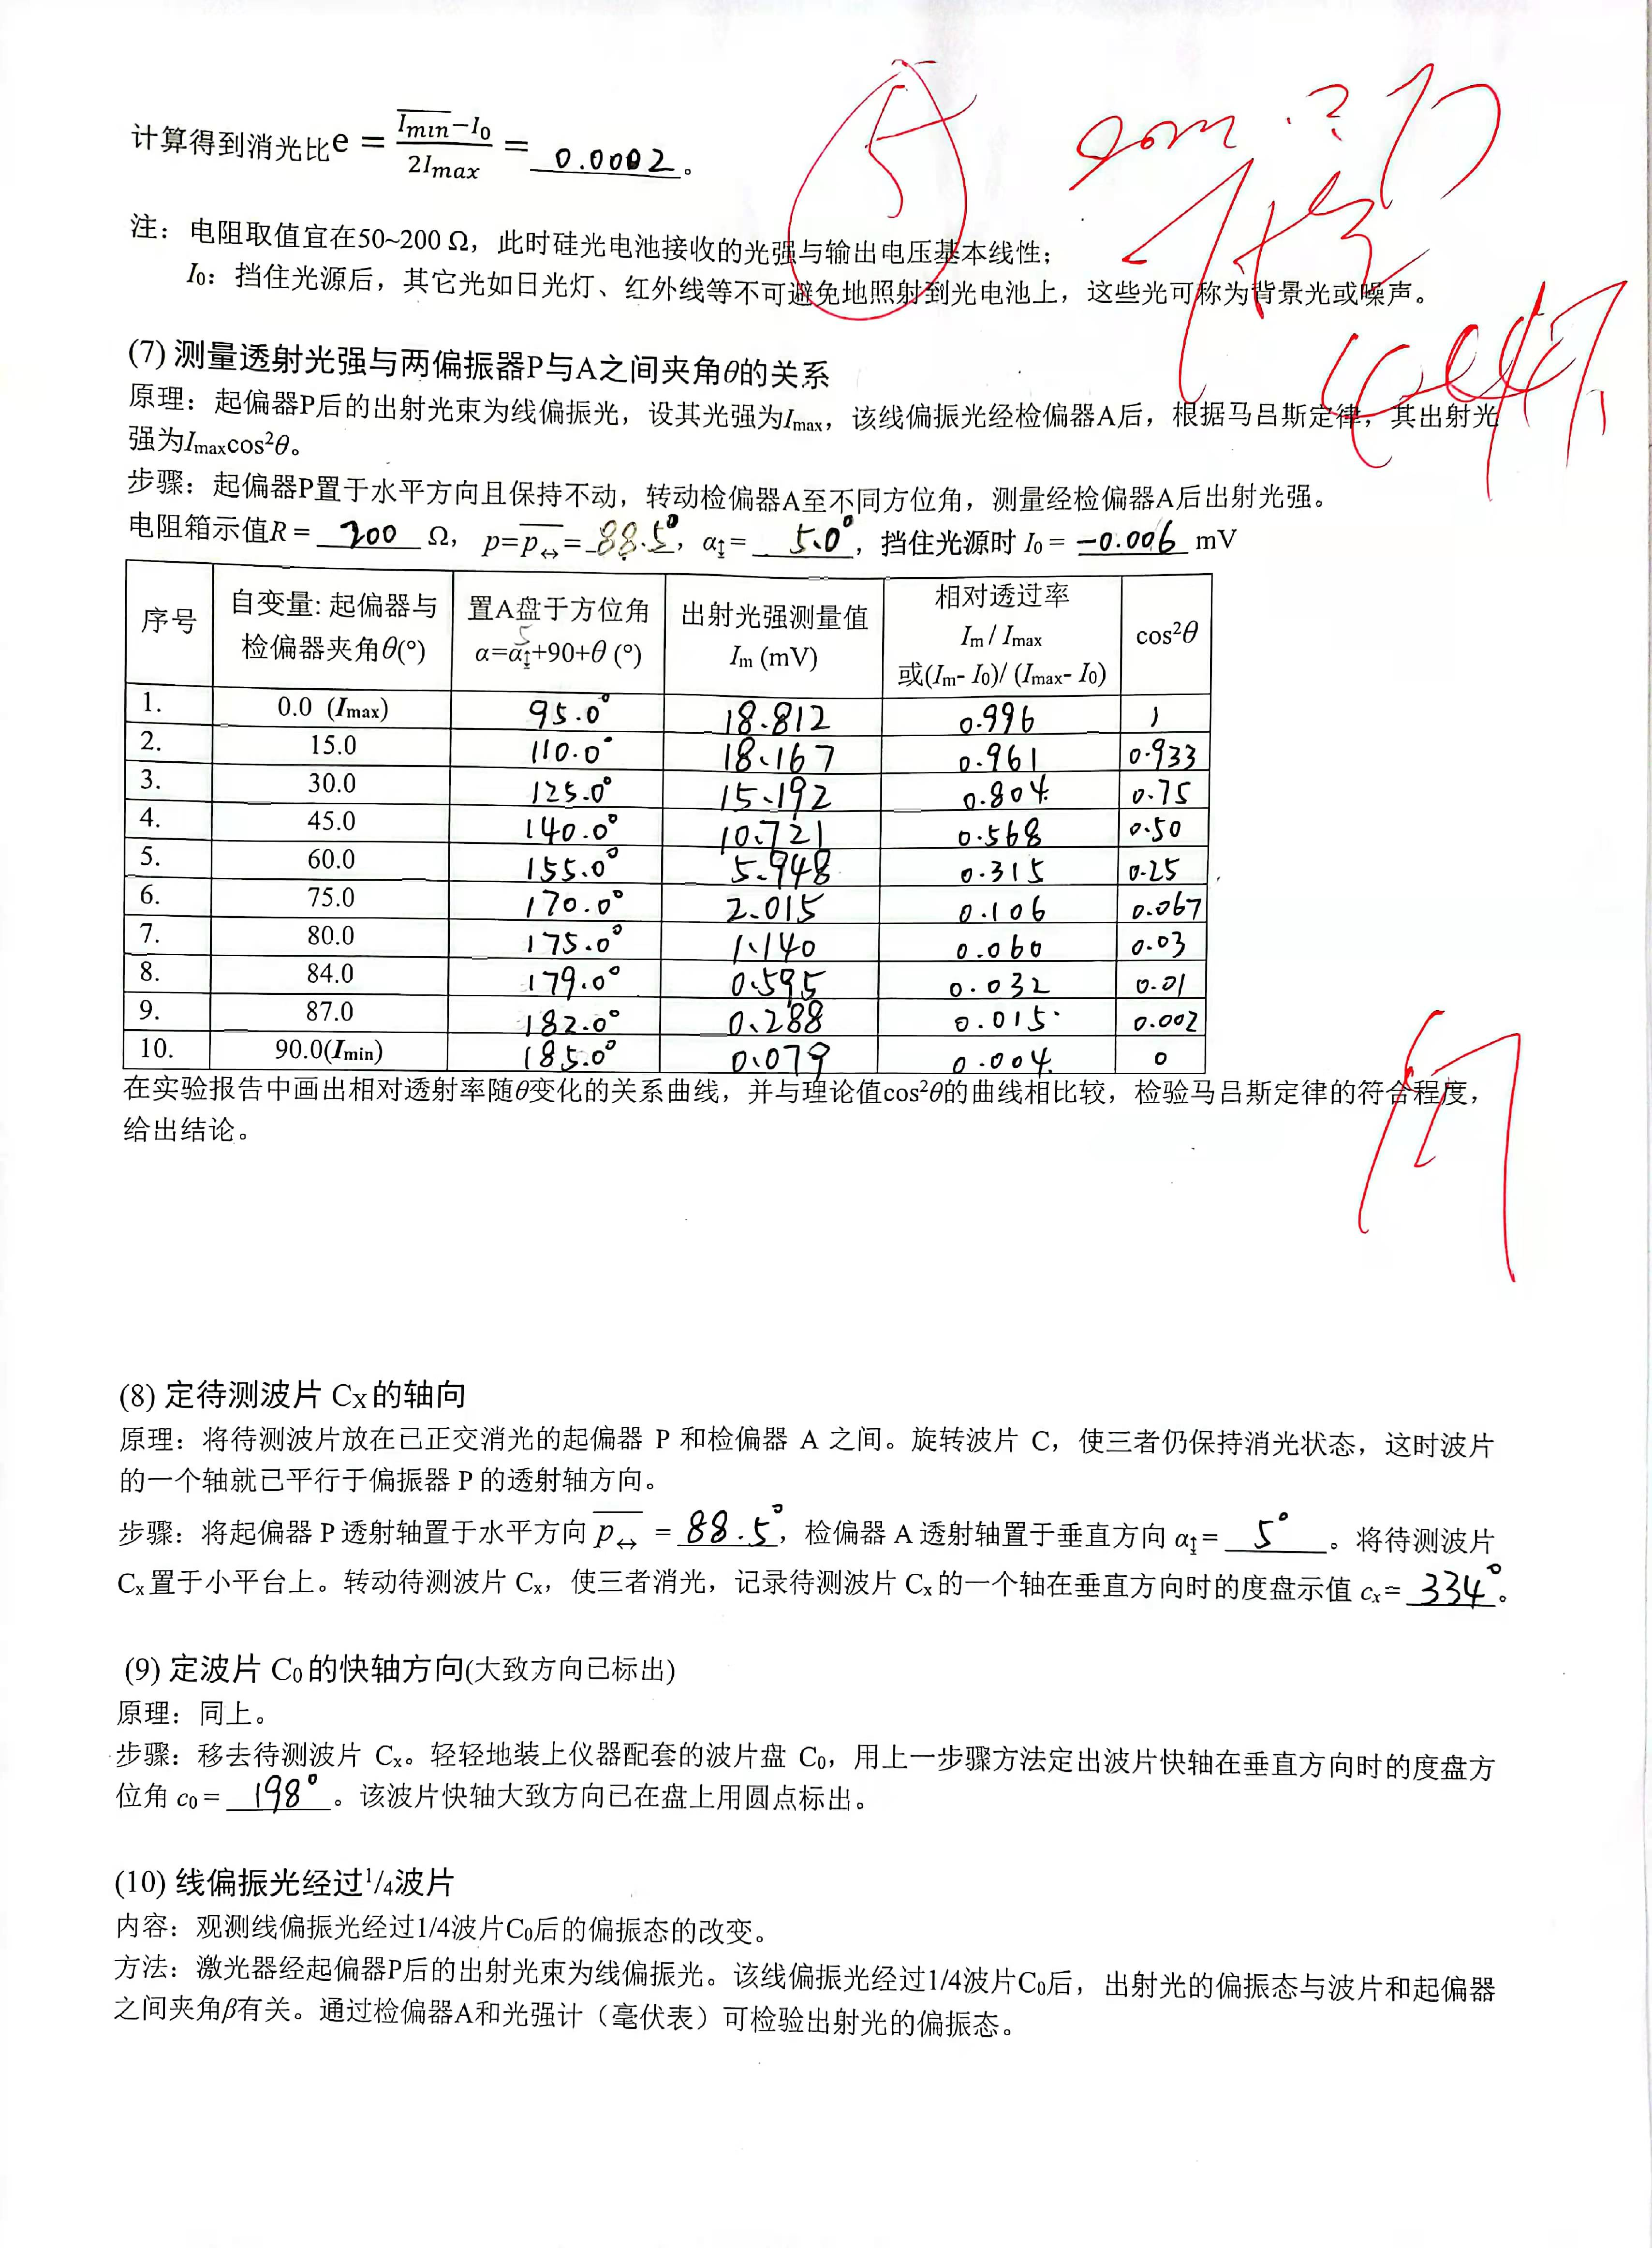
\includegraphics[scale=0.13]{2.jpg}
\end{figure}

\begin{figure}[H]
  \centering
  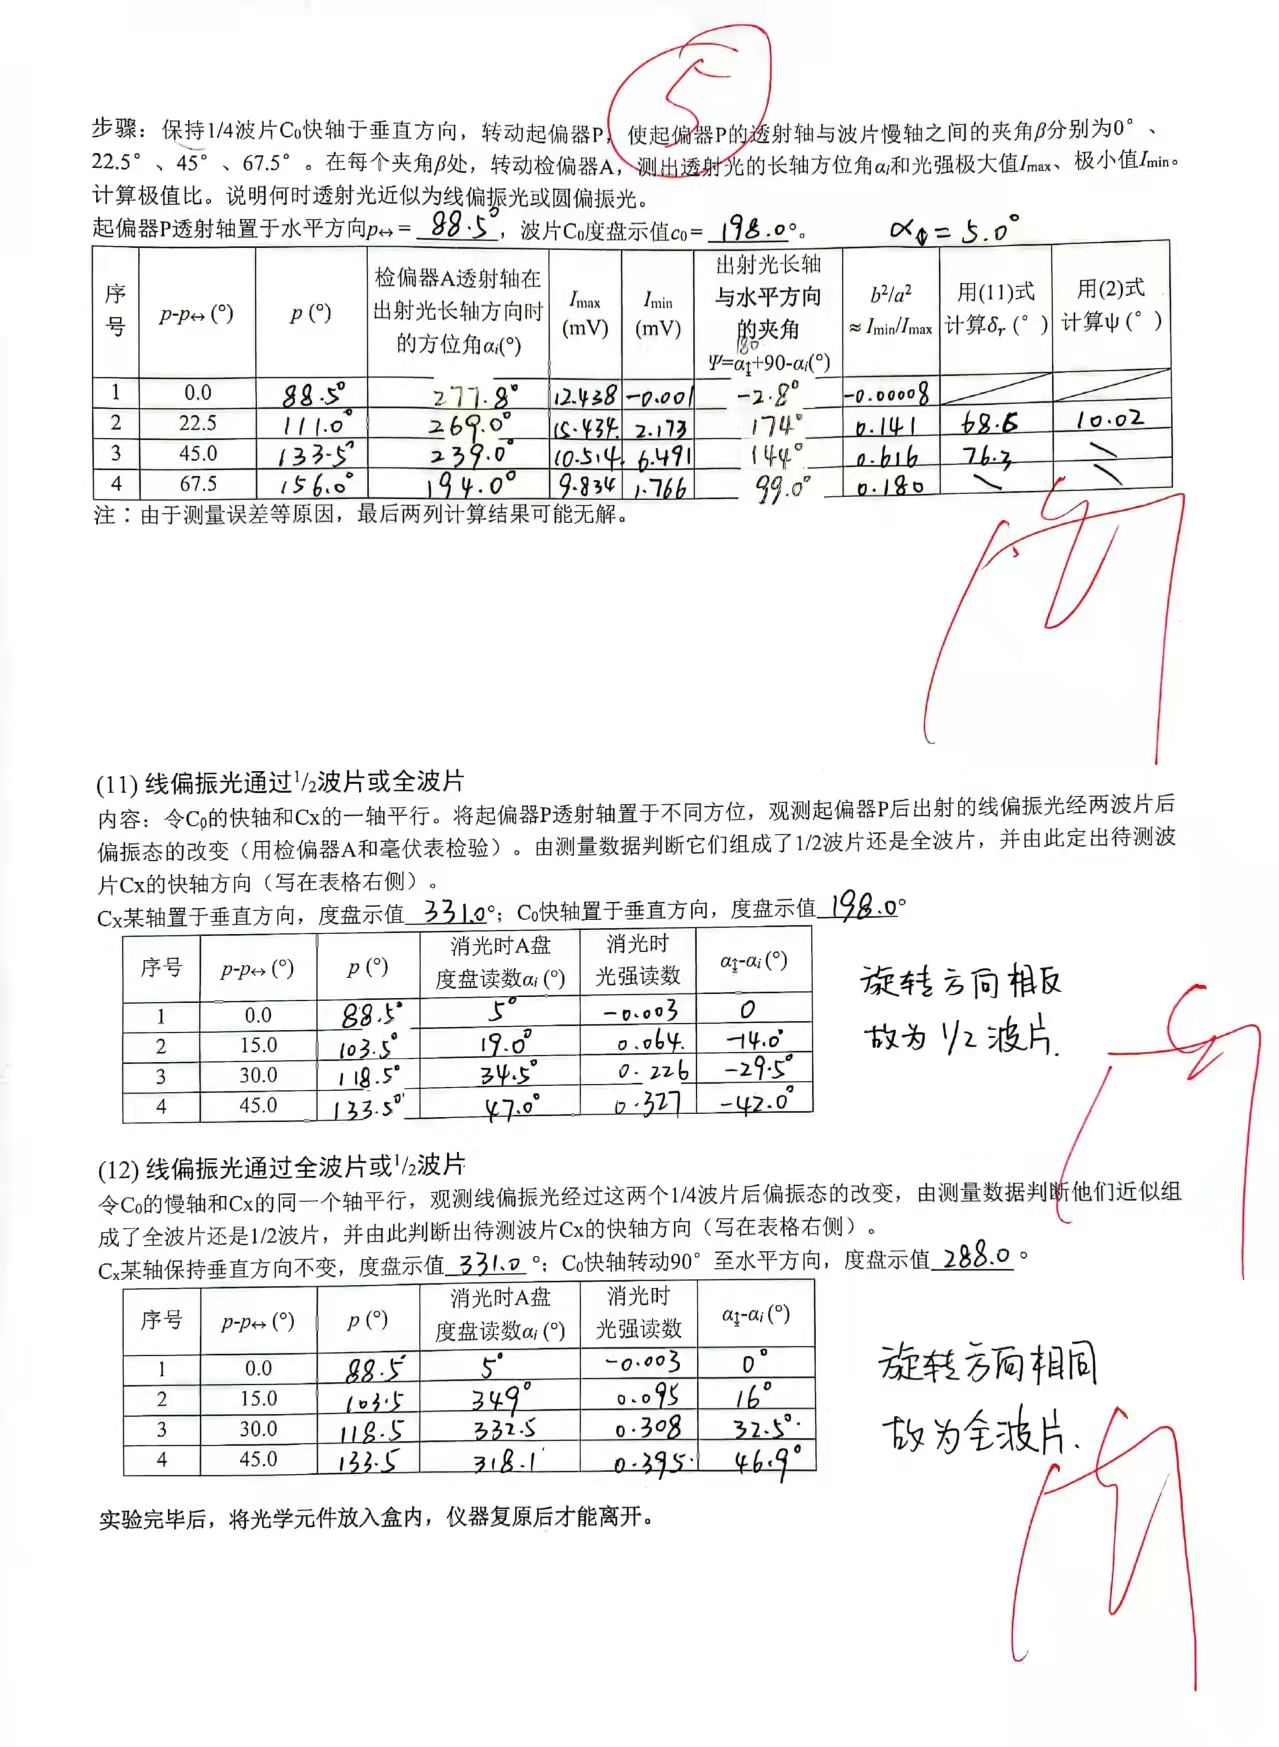
\includegraphics[scale=0.35]{3.jpg}
\end{figure}









\section{预习思考题}

\begin{figure}[H]
  \centering
  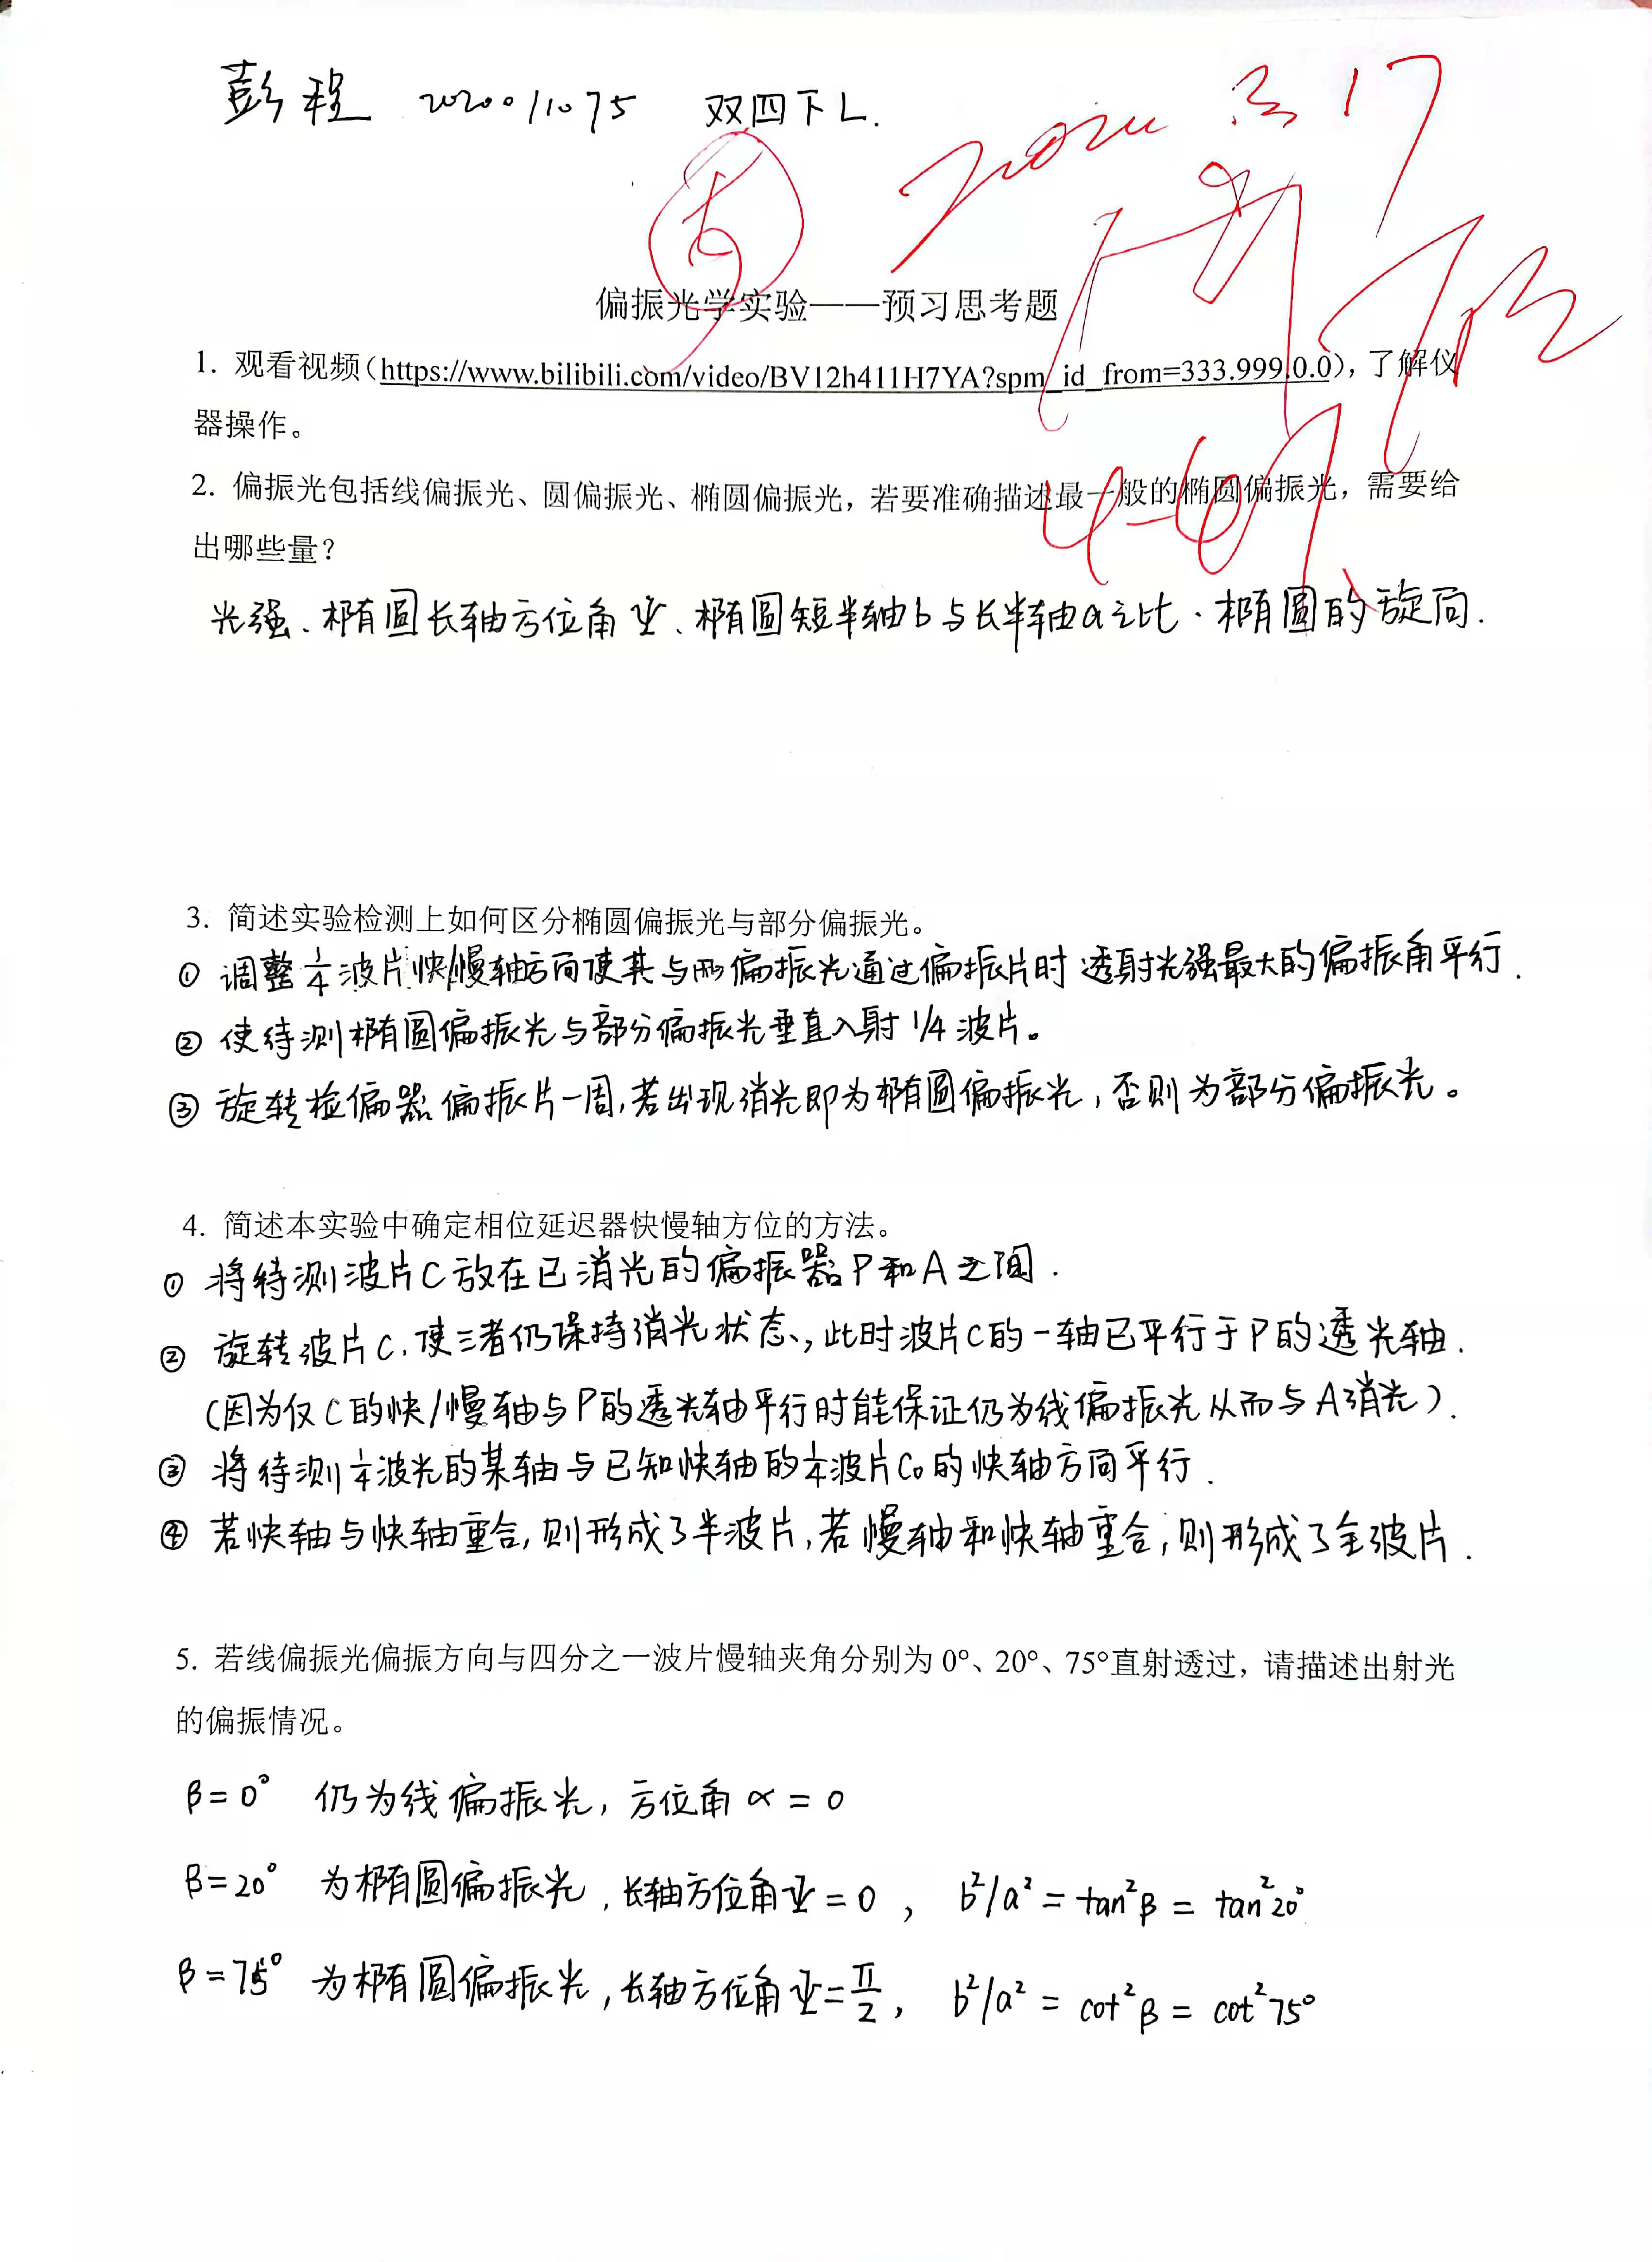
\includegraphics[scale=0.13]{4.jpg}
\end{figure}




\end{document}